% Pacotes e configurações padrão do estilo ``article''\
% -------------------------------------
\documentclass[a4paper,11pt]{article}
% Layout
% ------------------------------------------------------------------------------
%     Gráficos e layout ----------------------------------------------------------------------

\ifx\pdfmatch\undefined
\else
    \usepackage[T1]{fontenc}
    \usepackage[utf8]{inputenc}
\fi
% xetex:
\ifx\XeTeXinterchartoks\undefined
\else
    \usepackage{fontspec}
    \defaultfontfeatures{Ligatures=TeX}
\fi
% luatex:
\ifx\directlua\undefined
\else
    \usepackage{fontspec}
\fi
% End engine-specific settings

%      Fonte --------------------------------------------------------------------------------
%\usepackage{lmodern}
\usepackage{times}
%     Pacotes adicionados -------------------------------------------------------------------
\usepackage{ae}
%     Língua e hifenização ------------------------------------------------------------------
\usepackage[portuguese]{babel}
\usepackage{hyphenat}
%      Outros --------------------------------------------------------------------------------
\usepackage{hyperref} % Permite Links personalisados usando hyperref
\usepackage{fancyhdr}
\usepackage{sectsty}
\usepackage{float}   % Gerencia melhor o posicionamento das figuras e tabelas
%\usepackage{graphicx}
\usepackage[pdftex]{color,graphicx}
\usepackage{hyperref}
\usepackage{enumerate} % Permite alterar Layout do enumerate
%\usepackage{pdflscape}  % Permite alterar a orientação da pagina para Paisagem
%\usepackage{ifthen}  % Permite usar condicionais ifelse
%\usepackage[table]{xcolor} % Permite alterar as cores das células de uma tabela
\usepackage{amsmath,amssymb} % Ambiente para uso de elementos matemáticos
\usepackage{caption}
\usepackage{subcaption} % permite o uso de multiplas figuras com legenda (ambiente subfigure)
%\usepackage{minted} % Ambiente minted para colorir código de programas
\usepackage{natbib} % Para referencia bibliográfica
\usepackage{url}    % Referência de links na internet
%\usepackage{listings} % pacote para apresentar código de programação
\usepackage{indentfirst}  % Para indentar o primeiro parágrafo de cada seção
\usepackage{titling}  % Permite Montar uma página de titulo própria

% Layout do documento ------------------------------------------------------------------------
%     Bordas e tamanho da página ------------------------------------------------------------
\usepackage{geometry} 
 \geometry{ % Padrõa ABNT para relatórios
 a4paper,
 left=30mm,
 right=20mm,
 top=30mm,
 bottom=20mm
 }
%     Cabeçalho e Rodapé ---------------------------------------------------------------
\pagestyle{fancy}
  \lhead{}
  \chead{}
  \rhead{}
  \lfoot{}
  \cfoot{}
  \rfoot{\thepage}
%     Númeração ------------------------------------------------------------------------
  \pagenumbering{arabic}
%     Retas do cabeçalho e rodapé ------------------------------------------------------
  \renewcommand{\headrulewidth}{0.5pt}
  \renewcommand{\footrulewidth}{0.5pt}
%     Tamanho da letra de seções e derivadas --------------------------------------------
  \sectionfont{\normalsize}
  \subsectionfont{\small}
%     Hiperlinks ------------------------------------------------------------------------
  \hypersetup{
                  colorlinks,
                  citecolor=black,
                  filecolor=black,
                  linkcolor=black,
                  urlcolor=black
                  }
%     Definições do pdf ----------------------------------------------------------------------
\hypersetup{
    unicode=false,          % non-Latin characters in Acrobat’s bookmarks
    pdftoolbar=true,        % show Acrobat’s toolbar?
    pdfmenubar=true,        % show Acrobat’s menu?
    pdffitwindow=false,     % window fit to page when opened
    pdfstartview={FitH},    % fits the width of the page to the window    
    pdfauthor={Rafael Lima},     % author
    pdfnewwindow=true      % links in new window
}
%     Outros ----------------------------------------------------------------------------
      %\renewcommand{\thesection}{(\alph{section})} % muda o estilo de númeração das sections
      % alterando a formatação dos numeradores de lista de itens
      \renewcommand\theenumi{\arabic{enumi}}
      \renewcommand\labelenumi{(\textit{\theenumi})}
	  \renewcommand\theenumii{\arabic{enumii}}
	  \renewcommand\labelenumii{(\textit{\theenumi.\theenumii})}
      
% ---------------------------------------------------------------------------------------


%\usepackage{circuitikz}
\usepackage[makestderr]{pythontex}

\title{Laboratório 5} % Define o título do Relatório
\author{Rafael Lima}

% Definições Auxiliares ( Macros próprias )
% ------------------------------------------------------------------------------
%\input{relat_aux.tex} % Arquivo com minhas macros
\newcommand{\npy}[1]{\sympy{round(#1,4)}}
% ----------------------------------~>ø<~---------------------------------------
\begin{document}
% Capa e Índice ----------------------------------------------------------------
%--------------------------------------------------- Capa --------------------------------------------
%\newpage
\begin{figure}[h!]
\centering

\includegraphics[scale=0.9]{img/simb_unb.png}
\label{fig:unb}
\end{figure}

\begin{center}
{\LARGE Universidade de Brasília}\\
Departamento de Engenharia Elétrica\\
Professor: Henrique Cezar Ferreira\\
Disciplina: Controle Digital\\
\end{center}


\vspace{0.18\textheight}

\begin{center}
    \Huge \textbf{\\\thetitle \\}
\end{center}

\vspace*{\fill} % Completa espaço em branco e empurra o resto para o final da página

% Tabela com os nome das pessoas do grupo

\begin{table}[H]
    \begin{tabular}{ll}
        % Nome      & Matrícula
        Rafael Lima & 10/0131093 \\
    \end{tabular}
\end{table}

\vspace{0.5cm}

\begin{center}
    \textbf{Brasília\\
    \the\year} % Coloca o Ano atual
\end{center}

\thispagestyle{empty} % Retira o cabeçalho e o rodapé da página

% ------------------------------------------------- Índice -------------------------------------------
\newpage
\tableofcontents
\newpage
% ----------------------------------------------------------------------------------------------------

 % Capa para UnB
% Conteúdo ---------------------------------------------------------------------

\section{Projeto de Controlador Deadbeat}

% Código fonte colocado a parte para facilitar validação dentro do ipython
\begin{sympycode}
# Get Source Code
sys.path.insert(1, '../../')
from src.python.exsim5 import *
\end{sympycode}


\subsection{Controlador com erro zero para degrau unitário}

Dado o sistema definido pela seguinte função de tranferência:

\begin{equation}\label{eq:ex5-g1}
    G(z) = \frac{b(z)}{a(z)} = \sympy{sG1}
\end{equation}

Com a seguinte estrutura em malha fechada, em que $G_c(z)$ é um controlador discreto.

\begin{equation}
    M(z) = \frac{G_c(z)G(z)}{1 - G_c(z)G(z)}
\end{equation}

Para um controlador \textit{deadbeat} é buscado o erro zero para uma determinada entrada em tempo finito. Para tal podemos definir a função de transferência de malha fechada $M_1(z)$ desejada:

\begin{equation}\label{eq:ex5-gmf1}
    M(z) = \frac{A(z)}{z^n}
\end{equation}

Aplicando o teorema do valor final temos que o erro em regime permanente para a resposta ao degrau é dado por

$$E_{ss} = lim_{z \rightarrow 1}(z - 1)\frac{A(z)}{z^n}\frac{z}{(z-1)}$$

A partir do qual temos que $E_{ss} = 1 \Leftrightarrow A(z) = 1$. Assim podemos escolher $A(z) = 1$ para uma resposta em tempo mínimo, de modo que teremos uma resposta deadbeat no instantes amostrados. No entanto esta escolha acaba tendo como efeito a presentação de oscilação entre o instantes amostrados. Para evitar este problema foi adotado $A(z) = \frac{b(z)}{b(1}$ que representa um função de transferência normalizada em $z=1$ com os mesmos zeros que $G_1(z)$. Em outras palavras será adotado um contralador que tenha como efeito apenas alterar a resposta em regime permanente e a localização dos polos em malha fechada mas que conserve os mesmos zeros que a planta sem controlador.Para isto, isolando $G_c(z)$ na equação \ref{eq:ex5-gmf1} obtemos

$$
    G_{c}(z) = \frac{1}{G(z)}\frac{M(z)}{1-M(z)}
$$

Como $G(z) = \frac{b(z)}{a(z)}$, logo para a resposta em malha fechada escolhida teremos

\begin{equation}\label{eq:ex5-gc1}
    G_{c}(z) = \frac{a(z)}{b(z)}\frac{\frac{b(z)}{b(1)}}{z^n-\frac{b(z)}{b(1)}}
\end{equation}


Para que o sistema seja realizável é necessário que que $n \ge \#polos - \#zeros = 4  - 2 = 2$. Substituindo em \ref{eq:ex5-gmf1} temos

$$
M_1(z) = \sympy{roundExpr(sM1)}
$$

Substituindo $M(z) = M_1(z)$ na expressão \ref{eq:ex5-gc1}:

$$G_{c1}(z) = \sympy{roundExpr(sD1)}$$

Expandindo os termos:

$$G_{c1}(z) = \sympy{roundExpr(simplifyFraction(sD1))}$$

Colocando na forma fatorada destacando os zeros, polos e o ganho:

\begin{equation}
    G_{c1}(z) = \frac{z (z-0.219) (z-0.1793) (z-0.08059)}{(z-1) (z+0.1926) (z^2 + 0.8074z + 0.6255)}
\end{equation}

Com isto foi obtido a seguinte resposta ao degrau unitário:

\begin{figure}[H]
    \centering
    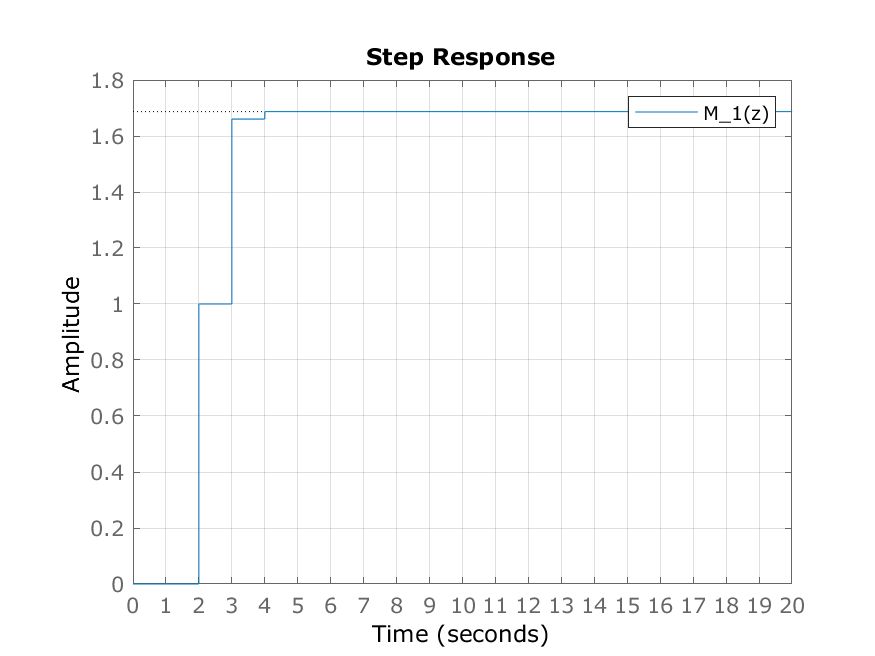
\includegraphics[width=0.6\linewidth]{img/exsim5-g1-deadbeat-sim.png}
    \caption{Resposta do Sistema para o controlador Deadbeat para sistema \ref{eq:ex5-g1}}
\end{figure}

\subsection{Controlador com erro zero para rampa unitária}

Dado um sistema definido pela seguinte função de transferência:

\begin{equation}\label{eq:ex5-g2}
    G_2(z) = \sympy{sG2}
\end{equation}

Procedendo de forma similar, foi adotado a seguinte resposta em malha fechada

$$
    M_2(z) = \frac{(n+1)z -n}{z^{n+1}}
$$

Temos que $n = \#polos - \#zeros + \#zeros = 3  - 2 + 2 = 1$, logo:

\begin{equation}\label{eq:ex5-g2}
    M_2(z) = \sympy{sM2}
\end{equation}

$$M_2(z) = \sympy{roundExpr(sM2)}$$

Substituindo $M(z) = M_2(z)$ na expressão \ref{eq:ex5-gc2}:

$$G_{c2}(z) = \sympy{roundExpr(sD2)}$$

Expandindo os termos:

$$G_{c2}(z) = \sympy{roundExpr(simplifyFraction(sD2))}$$

Colocando na forma fatorada destacando os zeros, polos e o ganho:

\begin{equation}
    G_{c2}(z) = \frac{5107.3 z (z-1)^2 (z-0.2865) (z+0.5)}{z (z+2.828) (z+1) (z+0.19)}
\end{equation}

A partir do qual foi obtido a seguinte resposta em malha fechada para a rampa unitária:

\begin{figure}[H]
    \centering
    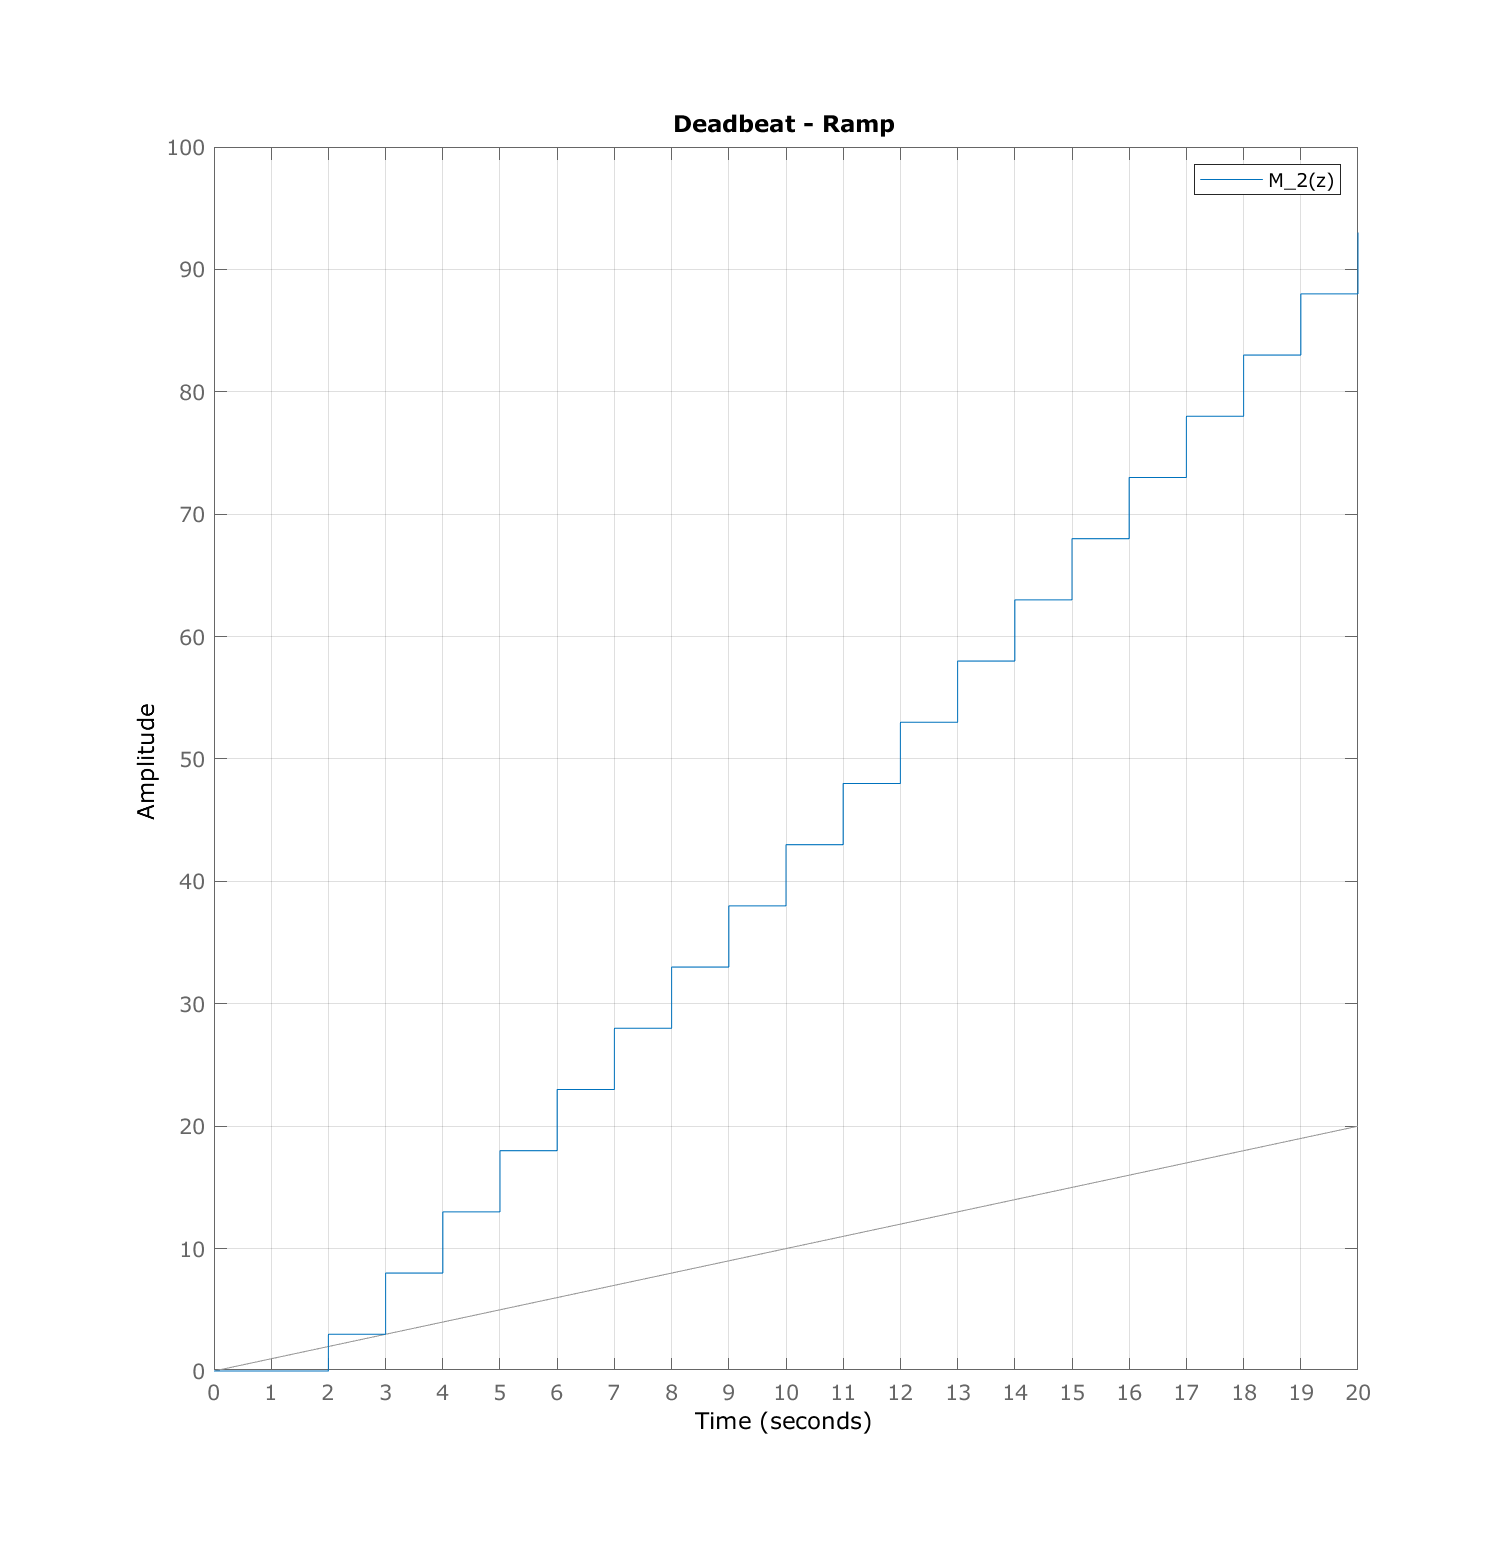
\includegraphics[width=0.6\linewidth]{img/exsim5-g2-deadbeat-sim.png}
    \caption{Resposta do Sistema para o controlador Deadbeat para sistema \ref{eq:ex5-g1}}
\end{figure}

\subsection{Comparação com outras técnicas de projeto}

O controlador \textit{deadbeat} traz vantagens e desvantagens conforme a aplicação desejada. Para verificar isto, será utilizado o projeto de controlador definido no Exercício de Simulação 2. O qual será novamente reproduzido aqui.

\subsubsection{Sistema em Malha Fechada}

Dado a função de tranferência de malha aberta $G(s)$

\begin{equation}
    G(s) = \frac{Y(s)}{U(s)} \sympy{G22}
\end{equation}

Em que

\begin{equation}
    U(s) = \sympy{G21}U_C(s) - \sympy{H22}Y(s)
\end{equation}

Aplicando o sinal de controle e fechando a malha obtemos:

$$G_{mf}(s) = \frac{Y(s)}{U_c(s)} = \sympy{G22mf}$$

Substituindo $a = \sympy{2*w0}$ e $b = \sympy{w0/2}$ temos

$$
G_{mf}(s) = \sympy{G22mf.subs([(a,2*w0),(b,w0/2)])}
$$
$$
G_{mf}(s) = \sympy{G22mf.subs([(a,2*w0),(b,w0/2),(kc,2*J*w0*w0/kp)])}
$$

Simplificando

\begin{equation}
    G_{mf}(s) = \sympy{simplifyFraction(G22mf.subs([(a,2*w0),(b,w0/2),(kc,2*J*w0*w0/kp)]),s)}
\end{equation}

\subsubsection{Discretização da Planta}

A discretização pode ser aproximada aplicando-se a transformada Z em conjunto de um segurador de ordem zero em série com o sistema. Desta forma temos $G_o(z) = Z(G_{zoh}(s)G(s)$ onde $G_{zoh}(s) = \frac{1-e^{-Ts}}{s}$. Aplicando as propriedades da transformada Z:

$$
\begin{array}{lcl}
    Z(\frac{1-e^{-Ts}}{s}G(z)) &=& Z(\frac{1}{s}G(z)) - Z(\frac{e^{-Ts}}{s}G(z))\\
    &=& Z(\frac{1}{s}G(z)) - (z^{-1})Z(\frac{1}{s}G(z))\\
    &=& (1 - z^{-1})Z(\frac{1}{s}G(z))\\
    &=& (1 - z^{-1})Z(\sympy{(1/s)*G22})\\
\end{array}
$$

Logo

\begin{equation}\label{eq:ex5-partialfrac}
 G(z) =   (1 - z^{-1})Z(\sympy{G22/s})
\end{equation}

Pela tabela temos que a transformada z de \ref{eq:ex5-partialfrac} é

$$G(z) = \sympy{Gz22} = \sympy{sGz22}$$
$$G(z) = \frac{T^2 k_{P}}{2J}\frac{z(1+z^{-1})}{z^2(1-z^{-1})^2}$$

\begin{equation}
    G(z) =\left(\frac{T^2 k_{P}}{2J}\right)\frac{z^{-1}(1+z^{-1})}{(1-z^{-1})^2}
\end{equation}

Como $G(z) = \frac{Y(z)}{U(z)}$

$$
\frac{Y(z)}{U(z)} =\left(\frac{T^2 k_{P}}{2J}\right)\frac{(z^{-1} + z^{-2})}{(1 - 2 z^{-1} + z^{-2})}
$$

$$
 Y(z)\left(1 - 2 z^{-1} + z^{-2}\right)
 = \left(\frac{T^2 k_{P}}{2J}\right)U(z)\left(z^{-1} + z^{-2}\right)
$$

De modo que temos a seguinte equação de diferenças:
\begin{equation}
 Y[k] +  2Y[k -1] +  Y[k - 2]
 = \left(\frac{T^2 k_{P}}{2J}\right)\left(U[k -1] +  U[k - 2]\right)
\end{equation}

\subsubsection{Função Transferência de malha fechada}

Dado a seguinte equação de diferenças do sinal de controle

\begin{equation}
    u[k] = t_0 u_C[k] - s_0 y[k] - s_1 y[k-1] - r_1 u[k -1]
\end{equation}

Usolando os termos de $u[k]$ e aplicando a transformada Z:

$$u[k] + r_1 u[k -1] = t_0 u_C[k] - s_0 y[k] - s_1 y[k-1]$$
$$U(z) + r_1 z^{-1}U(z) = t_0 U_C(z) - s_0 Y(z) - s_1 z^{-1}Y(z)$$

Agrupando os termos comuns e isolando $U(z)$:

$$U(z)\left(1 + r_1 z^{-1}\right) = t_0 U_C(z) - Y(z)\left(s_0 + s_1 z^{-1}\right)$$

\begin{equation}
U(z) = U_C(z)\frac{t_0}{\left(1 + r_1 z^{-1}\right)} -
  Y(z)\frac{\left(s_0 + s_1 z^{-1}\right)}{\left(1 + r_1 z^{-1}\right)}
\end{equation}

Substuindo:

$$
    Y(z) =\left(\frac{T^2 k_{P}}{2J}\right)\frac{z^{-1}(1+z^{-1})}{(1-z^{-1})^2}U(z)
$$
$$
    Y(z) = \left(\frac{T^2 k_{P}}{2J}\right)\frac{z^{-1}(1+z^{-1})}{(1-z^{-1})^2}\left( U_C(z)\frac{t_0}{\left(1 + r_1 z^{-1}\right)} - Y(z)\frac{\left(s_0 + s_1 z^{-1}\right)}{\left(1 + r_1 z^{-1}\right)}\right)
$$

$$
    Y(z)\left(1 + \frac{\left(s_0 + s_1 z^{-1}\right)}{\left(1 + r_1 z^{-1}\right)}\right)
= U_c(z)\left(\frac{T^2 k_{P}}{2J}\right)\left(\frac{z^{-1}(1+z^{-1})}{(1-z^{-1})^2}\right)\left( \frac{t_0}{\left(1 + r_1 z^{-1}\right)}\right)
$$

De forma que a função em malha fechada com o controlador fica:

$$
    \frac{Y(z)}{U_c(z)} = \left(\frac{T^2 k_{P}}{2J}\right)\frac{\left(\frac{z^{-1}(1+z^{-1})}{(1-z^{-1})^2}\right)\left( \frac{t_0}{\left(1 + r_1 z^{-1}\right)}\right)}{\left(1 + \frac{\left(s_0 + s_1 z^{-1}\right)}{\left(1 + r_1 z^{-1}\right)}\right)}
$$

$$
    \frac{Y(z)}{U_c(z)} = \left(\frac{T^2 k_{P}t_0}{2J}\right)
    \frac{
        z^{-1}(1+z^{-1})
    }{
        (1-z^{-1})^2 \left((1 + r_1 z^{-1}) + \left(s_0 + s_1 z^{-1}\right)\right)
     }
$$

\begin{equation}
    \frac{Y(z)}{U_c(z)} = \left(\frac{T^2 k_{P}t_0}{2J}\right)
    \frac{
        z^{-1}(1+z^{-1})
    }{
        (1-z^{-1})^2 \left((1 + s_0) + (r_1 + s_1) z^{-1}\right)
     }
\end{equation}

\subsubsection{Controladores}

Dado o sistema definido abaixo

\begin{figure}[H]
    \centering
    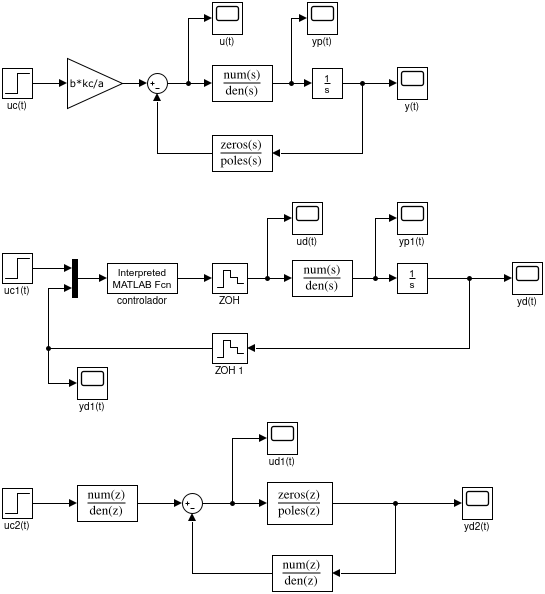
\includegraphics[width=0.9\linewidth]{img/exsim5model.png}
    \caption{Diagrama de Blocos do Sistema no Simulink - Planta exsim5}
\end{figure}

\subsubsection{Comparação Controle Deadbeat vs Controle Discratizado}

Para o fins de comparação foi adotado a seguinte diagrama para o controle projetados para o exercício de simulação 2:

\begin{figure}[H]
    \centering
    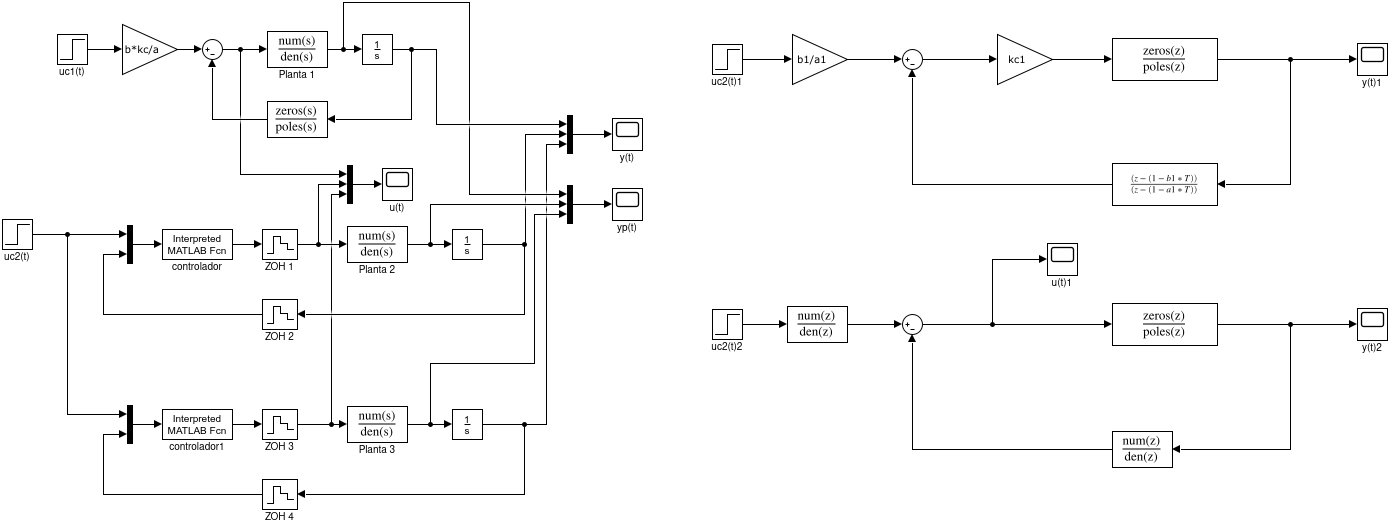
\includegraphics[width=1\linewidth]{img/exsim2model.png}
    \caption{Diagrama de Blocos do Sistema no Simulink - Planta exsim2}
\end{figure}

Com base nos valores definidos em script, foram obtidos os seguintes resultados para a simulação:

\begin{figure}[H]
    \centering
    \begin{subfigure}[m]{0.49\linewidth}
        \centering
        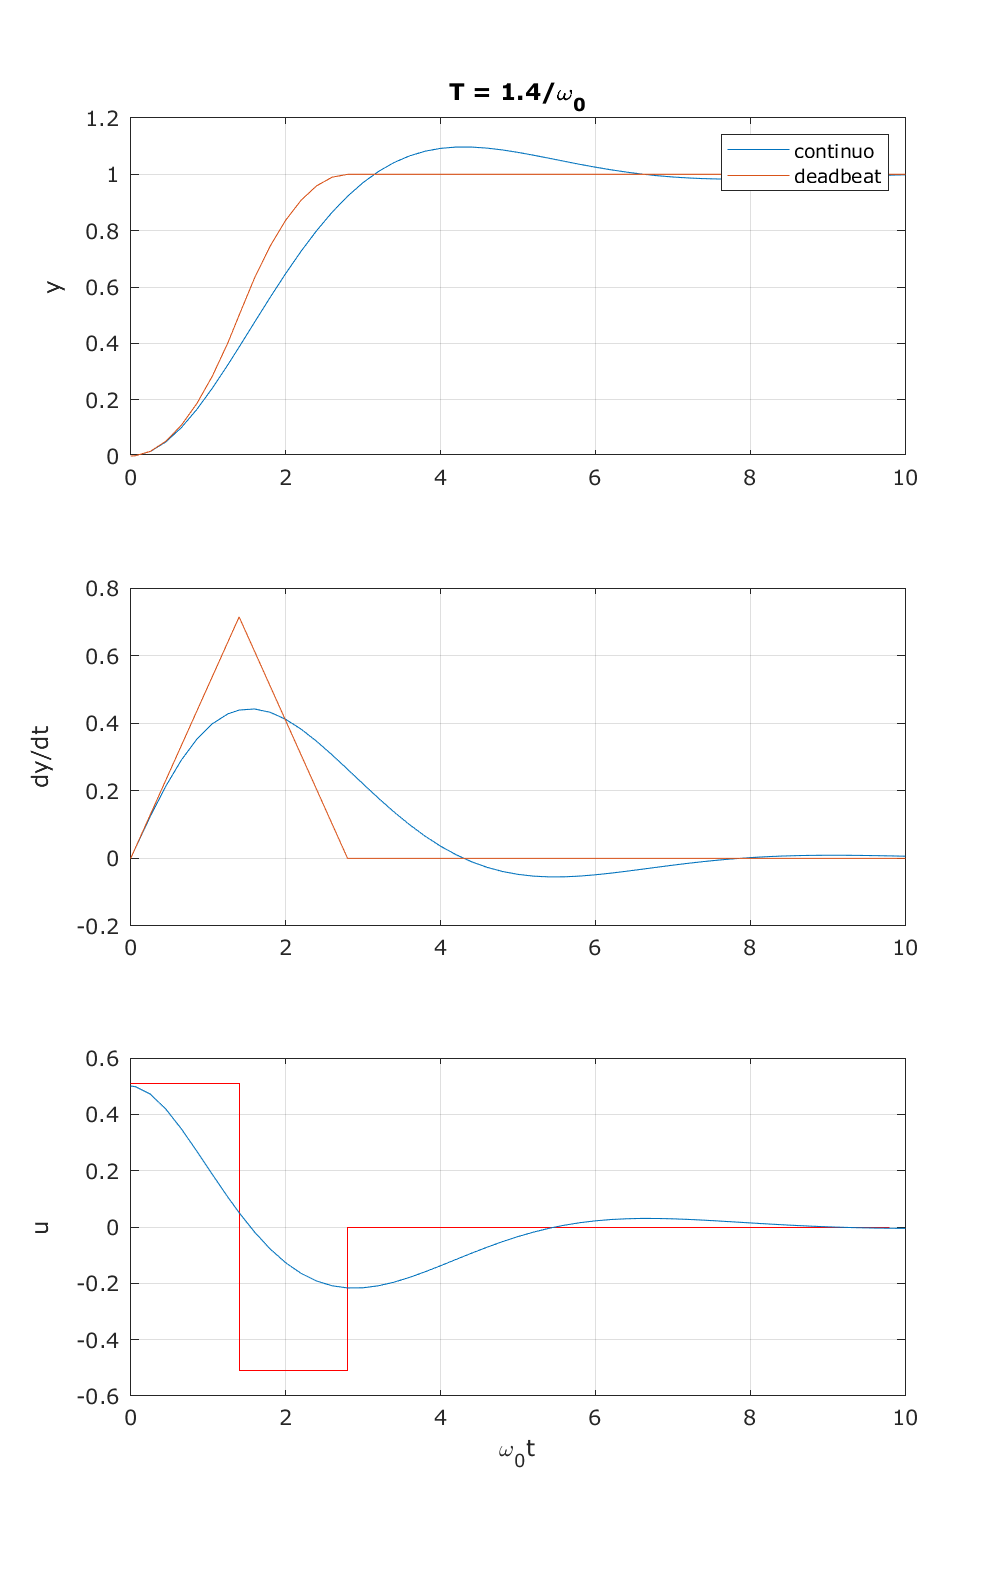
\includegraphics[width=1\linewidth]{img/exsim5-deadbeat-sim.png}
        \caption{Controlador Deadbeat - exsim5}
    \end{subfigure}
    \hfill
    \begin{subfigure}[m]{0.49\linewidth}
        \centering
        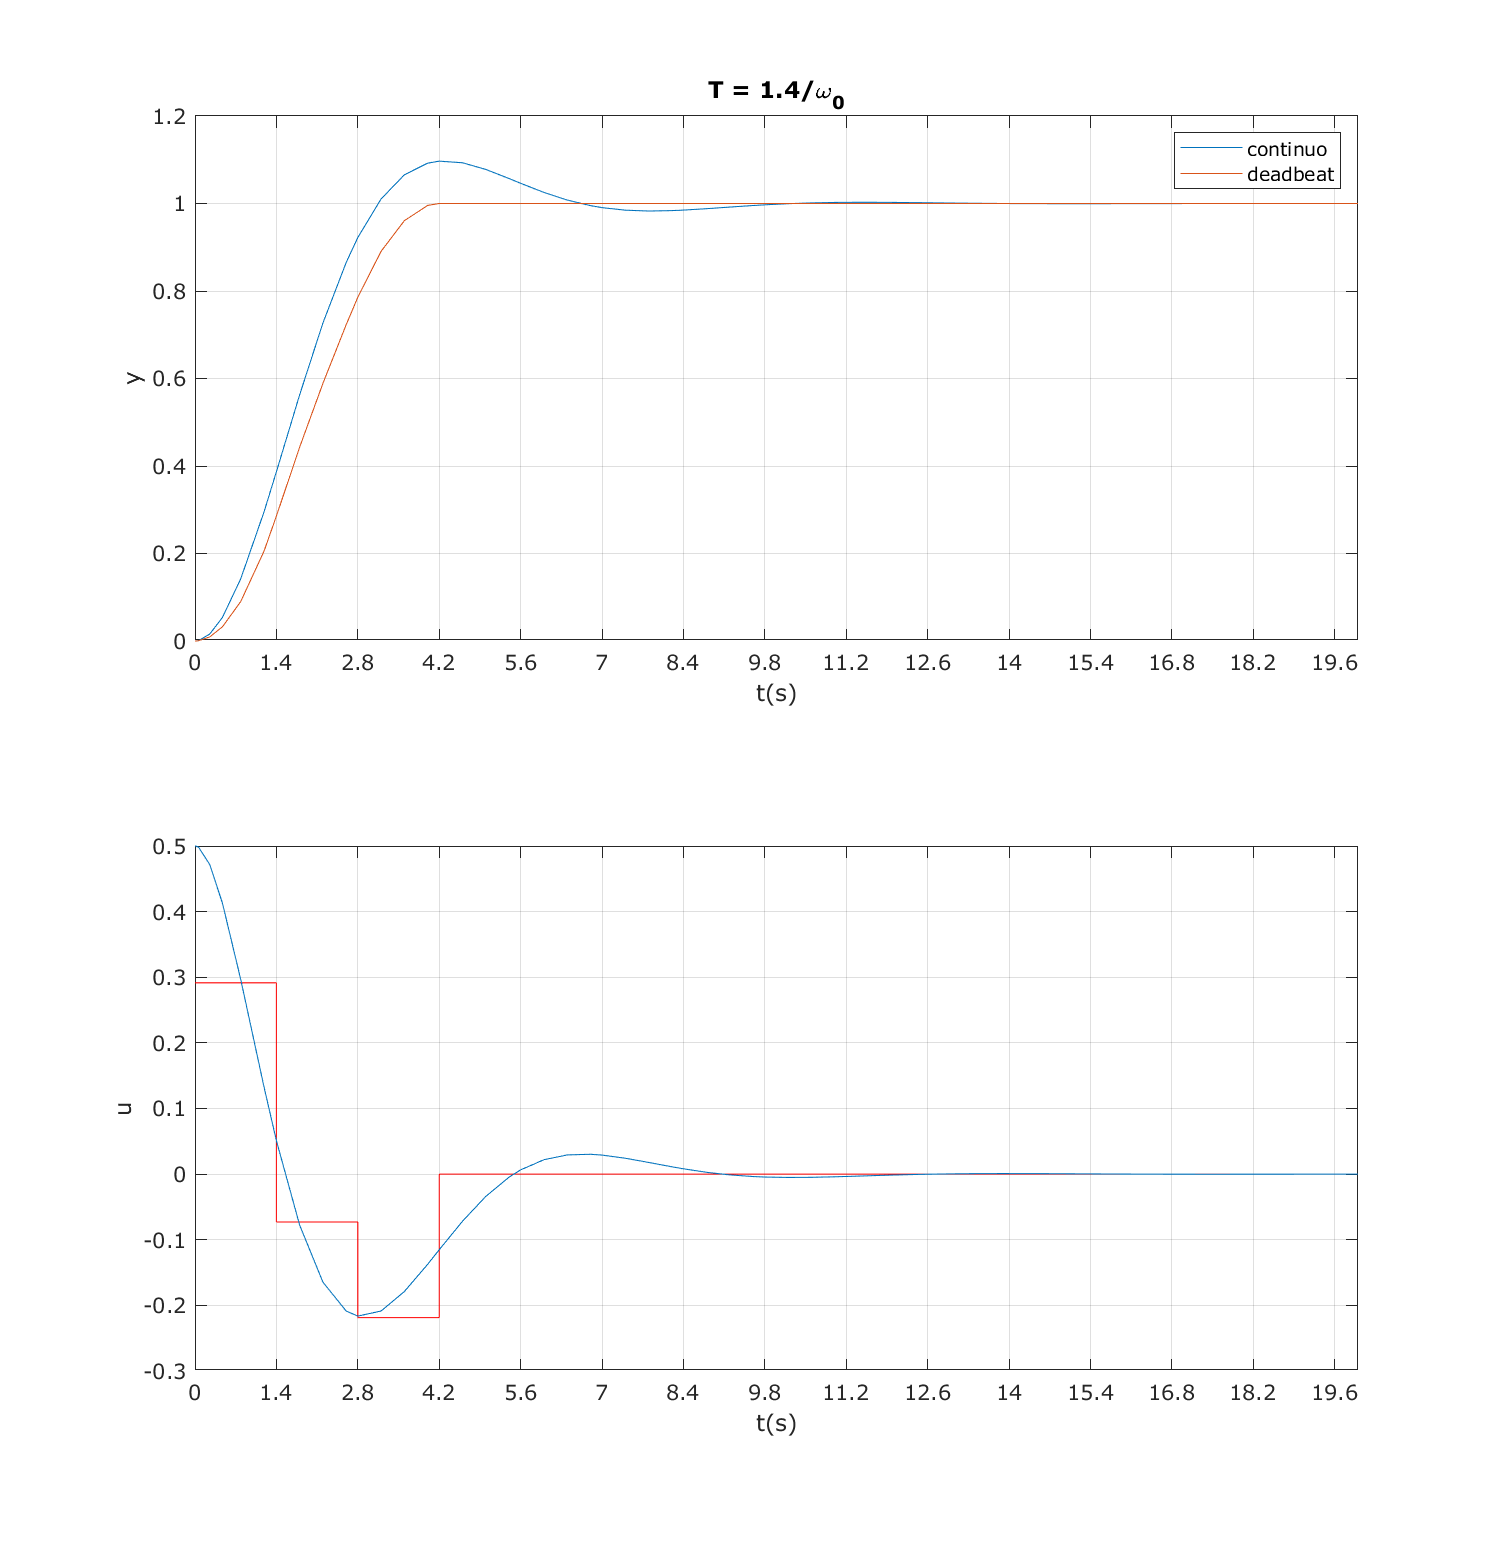
\includegraphics[width=1\linewidth]{img/exsim5-exsim2-sim.png}
        \caption{Controlador Discretizado - exsim2}
    \end{subfigure}
\end{figure}

Comparando ambas simulações percebemos que a metodologia adotada para o projeto do controlador na lanta exsim2 acaba levando mais tempo para estabilizar e têm um atraso em relação ao sistema contínuo. Enquanto para o controle da planta exsim5 é percebido uma resposta mais rápida e também uma ação de controle bme mais agressiva para um mesmo tempo de amostragem contando com uma varição bastante brusca do sinal passado para a planta. Algo que é característico de controladores deadbeat.

\section{Conclusão}

O controlador deadbeat constitui uma opção interessante por garantir de em um tempo finito o erro $0$ em regime permanente para uma determinada entrada de referência. Constindo por tanto uma opção bastante interessante para projetos de posicionamento como servo mecanismos ao custo que acaba trazendo uma resposta bastante agressiva para o controlador, podendo provocar um desgate do atuador caso seja especificado tempos de amostragem muito curtos.

% ------------------------------------------------------------------------------
\newpage
% Referências
\addcontentsline{toc}{section}{Referências} % Adiciona linha no indice
\bibliographystyle{abbrv} % Define Estilo e gera bibliografia
\bibliography{references} % Adiciona Arquivo com Referências

% Acrescentadas no arquivo references.bib
% para usa-las no texto basta usar \citep{}
% para citar sem usar no texto basta usar \nocite{}
\nocite{sympy}
\nocite{pythontex}
\nocite{matlabcontrol}
\nocite{matlabsymbolic}
\nocite{ogata2010modern}

% ------------------------------------------------------------------------------
\newpage
\section*{Anexos}
\addcontentsline{toc}{section}{Anexos} % Adiciona linha no indice
\subsection*{Python}

Para os cálculos e demonstrações foi utilizado o pacote \textit{Python}\TeX\ \cite{pythontex} para o \LaTeX\ em conjunto da bibliteca \textit{sympy}\cite{sympy}. Segue o script completo em python:

\inputminted[xleftmargin=15pt,linenos,frame=single,framesep=5pt,breaklines=true]{python}{../python/exsim5.py}

\newpage
\subsection*{Matlab}

\subsubsection*{Parte 1}
Para o desenho dos gráficos e simulações foi utilizado o \textit{Matlab} em conjunto das toolbox \textit{Control System}\cite{matlabcontrol} e \textit{Symbolic Math}\cite{matlabsymbolic}. Segue o código referente usado

\inputminted[xleftmargin=15pt,linenos,frame=single,framesep=5pt,breaklines=true]{matlab}{../matlab/exsim5/exsim5.m}

\newpage
\subsubsection*{Parte 3 - Controlador Dead Beat}
Para avaliação da resposta do controlador Dead Beat foi utilizado uma versão modificada dos script \textit{exsim5script} em \textit{Matlab} fornecido pelo professor:
\inputminted[xleftmargin=15pt,linenos,frame=single,framesep=5pt,breaklines=true]{matlab}{../matlab/exsim5/exsim5script.m}

\newpage
\subsubsection*{Parte 3 - Controlador Discretizado}
Para comparativo com os resultados da simulação 2, foi utilizado uma versão modificada dos script \textit{exsim2script} em \textit{Matlab} fornecido pelo professor:
\inputminted[xleftmargin=15pt,linenos,frame=single,framesep=5pt,breaklines=true]{matlab}{../matlab/exsim5/exsim2script.m}



% ------------------------------------------------------------------------------
\end{document}
